内核可以视为提交执行的异步任务。这些任务必须提交到一个队列中,并安排在设备上执行。许多情况下,内核必须按照特定的顺序执行,才能计算出正确的结果。如果获得正确的结果需要任务A在任务B之前执行,那么任务A和B之间存在依赖关系。\par
 
然而,内核并不是调度的唯一形式。内核开始执行前,内核访问的任何数据都需要在设备上可用。这些数据依赖可以以数据任务的方式,从一个设备传输到另一个设备。数据传输任务可以是显式编码的拷贝操作,也可以是运行时执行的隐式数据移动。\par

如果把程序中的所有任务,以及存在的依赖关系画出来,就可以形成一个图。这个任务图是个有向无环图(DAG),其中节点是任务,边是依赖项。图是有向的,因为依赖是单向的:任务A必须发生在任务B之前。因为不包含从节点返回自身的循环或路径,所以无环。\par

图3-8中,A任务前必须执行任务B和C。同样地,B和C之前必须在D之前执行。而B和C没有依赖,运行时是可以以任何顺序执行(甚至并行)任务。因此,如果B和C能够同时执行,则这个图可能的法律次序是: A $\Rightarrow$ B $\Rightarrow$ C $\Rightarrow$ D, A $\Rightarrow$ C $\Rightarrow$ B $\Rightarrow$ D,甚至时A $\Rightarrow$ \{B,C\} $\Rightarrow$ D。\par

\hspace*{\fill} \par %插入空行
图3-8 简单的任务图
\begin{center}
	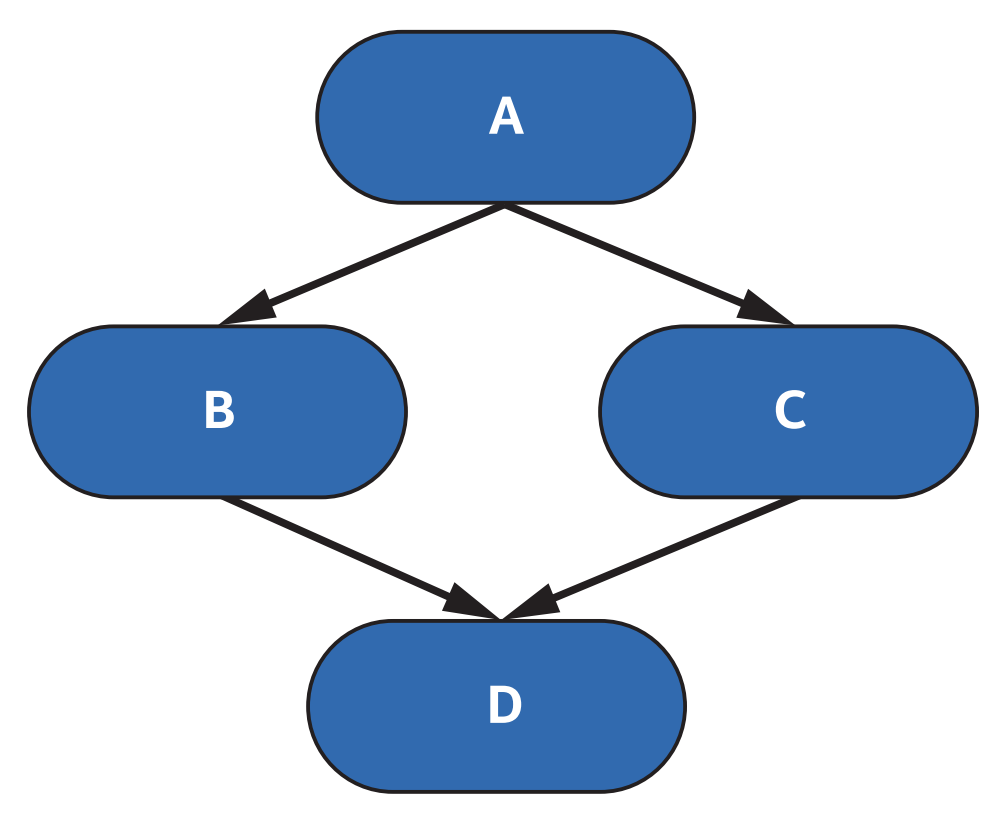
\includegraphics[width=0.6\textwidth]{content/chapter-3/images/4}
\end{center}

任务可能与所有任务的子集有依赖性,我们只指定与正确性有关的依赖项。这种灵活性为优化任务图的执行顺序提供了自由度。图3-9中,我们扩展了任务图图3-8,添加了E和F,并且E必须在F前执行。然而,任务E和F与节点A,B,C,D没有依赖性。这允许运行时可以选择序执行任务的顺序。\par

\hspace*{\fill} \par %插入空行
图3-9 不相交依赖关系的任务图
\begin{center}
	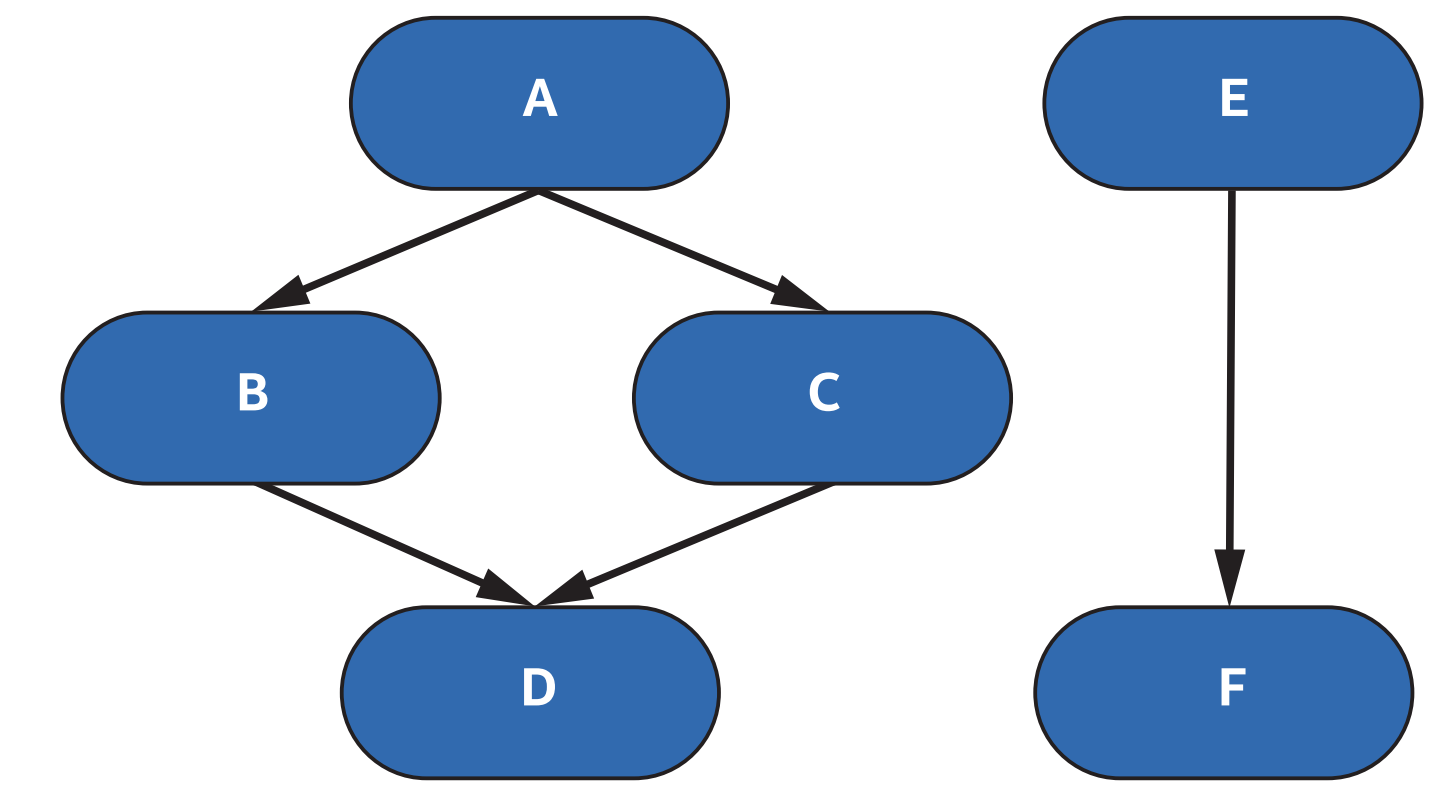
\includegraphics[width=0.8\textwidth]{content/chapter-3/images/5}
\end{center}

有两种不同的方法来为任务的执行(例如内核的启动)建模:队列可以按照提交的顺序执行任务,也可以按照自定义的依赖项的任意顺序执行任务。我们有几种机制来定义正确排序所需的依赖项。\par

\hspace*{\fill} \par %插入空行
\textbf{有序队列}

对任务进行排序的最简单方式是将它们提交给一个有序的队列对象。有序队列按照任务提交的顺序执行任务,如图3-10所示。尽管有序队列的任务排序非常简单,它的缺点是即使独立任务之间不存在依赖关系,任务的执行也将串行化。有序队列在启动应用程序时很有用,因为简单、直观、执行顺序确定,并且适用于许多代码。\par

\hspace*{\fill} \par %插入空行
图3-10 有序队列的使用方式
\begin{center}
	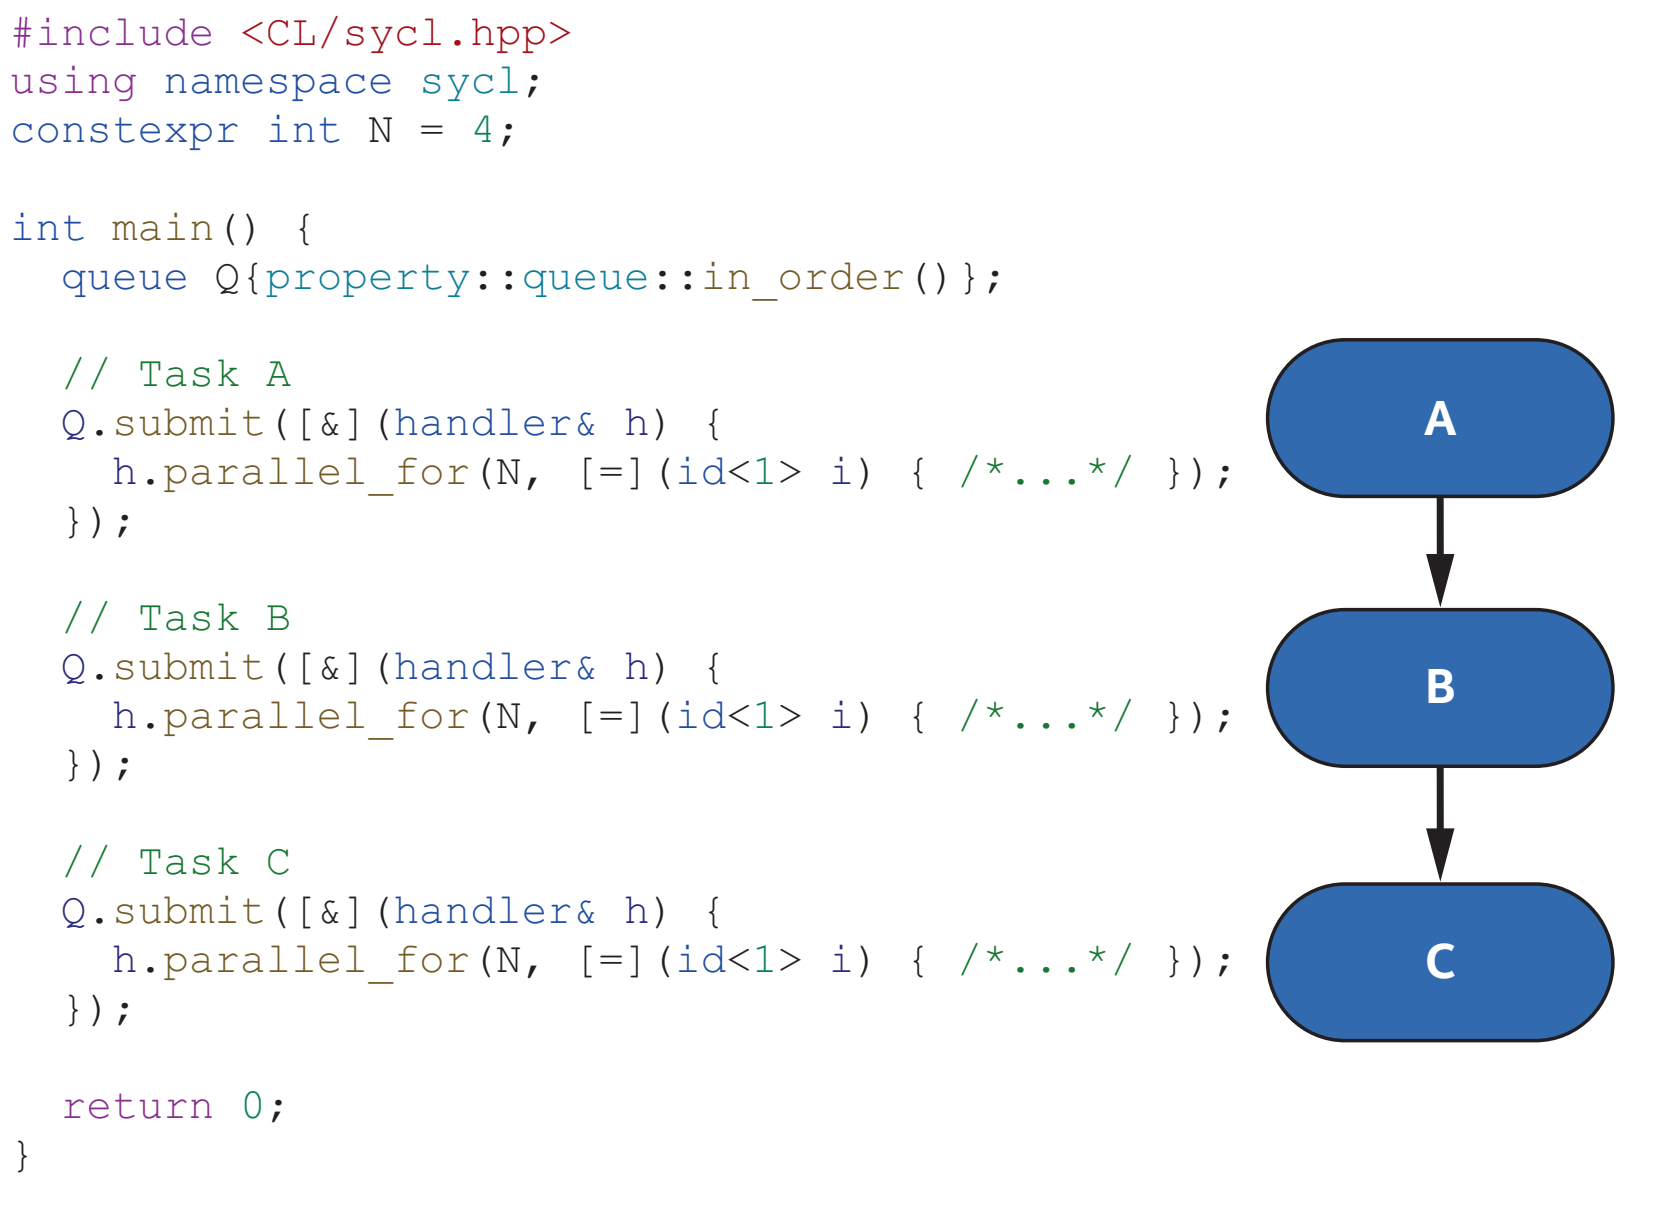
\includegraphics[width=1.0\textwidth]{content/chapter-3/images/6}
\end{center}

\hspace*{\fill} \par %插入空行
\textbf{无序队列}

由于队列是无序队列(除非使用有序队列属性创建),必须提供提交任务进行的排序方法。队列允许通知运行时任务间的依赖关系,从而对任务进行排序。并且,可以使用命令组显式或隐式地指定这些依赖项。\par

命令组是指定任务及其依赖关系的对象。命令组通常以C++ Lambda的形式,作为参数传递给队列对象的submit()。这里Lambda的唯一参数是对handler对象的引用。handler对象在命令组中用于指定操作、创建访问器和指定依赖项。\par

\hspace*{\fill} \par %插入空行
\textbf{事件的显式依赖}

任务之间的显式依赖关系就像我们已经看到的例子(图3-8),其中任务A必须在任务B之前执行,通过这种方式表达的依赖关系是显式的,并且基于计算,而不是数据。注意,表达计算之间的依赖关系,主要与使用USM有关,使用缓冲区的代码通过访问器表达大多数依赖关系。图3-4和图3-5中,只是告诉队列等待之前提交的所有任务完成后再继续,而我们可以通过事件对象表达任务的依赖关系。当向队列提交命令组时,submit()方法会返回一个事件对象,事件可以以两种方式使用。\par

首先,可以通过在事件上显式地调用wait()来进行同步。这迫使运行时等待生成事件的任务完成,才继续执行主机程序。显式地等待事件对于调试应用程序非常有用,但wait()会过度地限制任务的异步执行,因为阻塞主机线程上的所有执行,也可以在队列对象上调用wait(),这将阻塞主机上的执行,直到所有进入队列的任务都完成。\par

这就引出了使用事件的第二种方式。处理程序类包含一个名为depends\_on()的方法。此方法接受单个事件或事件组,并通知运行时所提交的命令组需要在执行命令组内的操作之前完成指定的事件。图3-11展示了如何使用depends\_on()来排序任务。\par

\hspace*{\fill} \par %插入空行
图3-11 使用事件和depends\_on
\begin{center}
	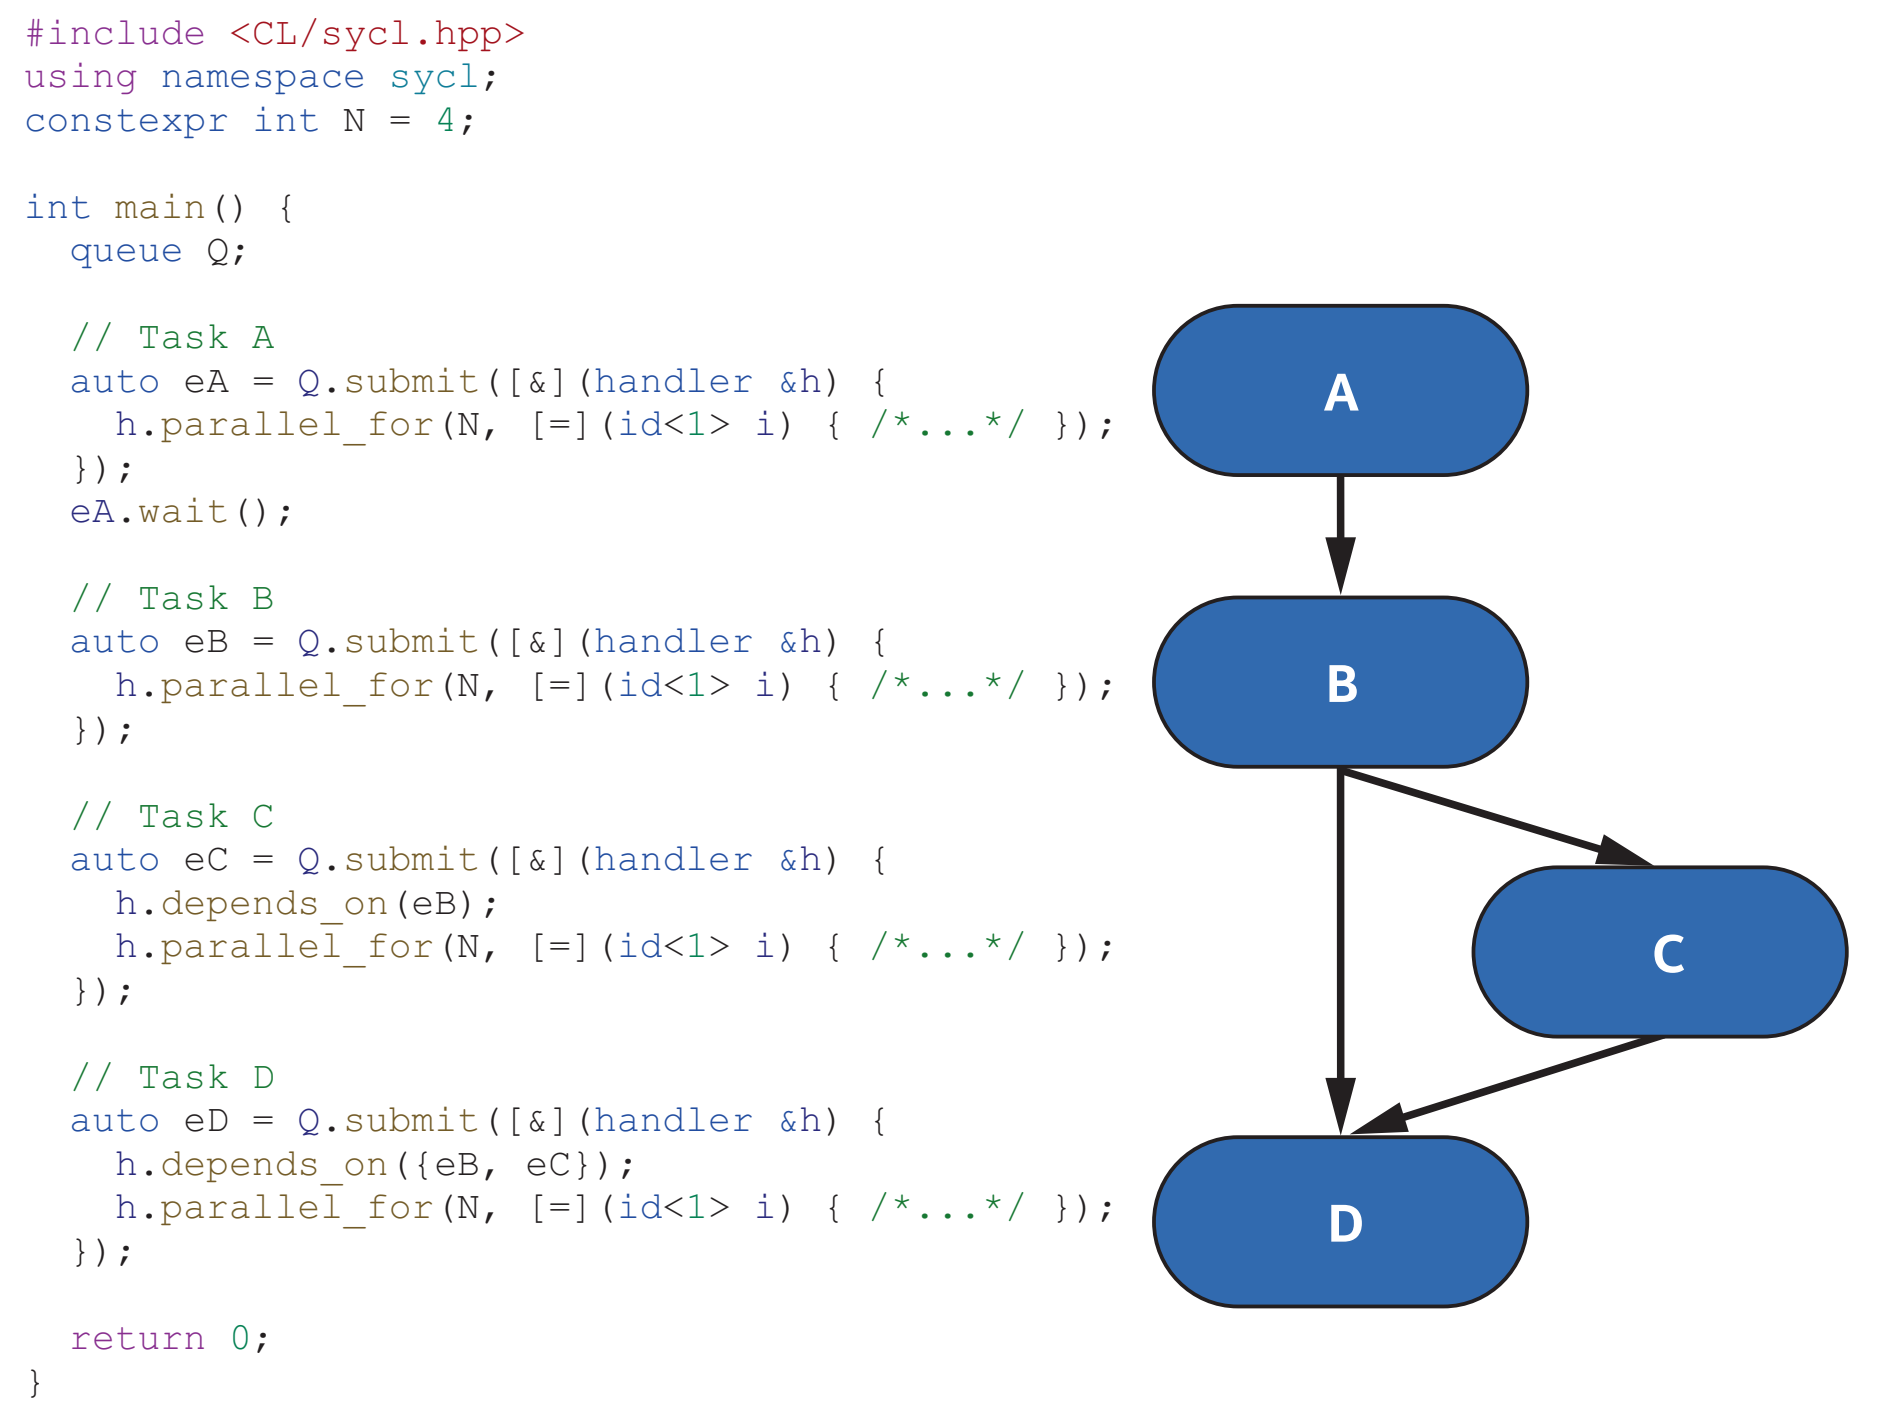
\includegraphics[width=1.0\textwidth]{content/chapter-3/images/7}
\end{center}

\hspace*{\fill} \par %插入空行
\textbf{访问器的隐式依赖}

任务之间的隐式依赖关系由数据依赖关系创建,任务之间的数据依赖有三种形式,如图3-12所示。\par

\hspace*{\fill} \par %插入空行
图3-12 三种的数据依赖关系
\begin{table}[H]
	\begin{tabular}{|c|c|}
		\hline
		\textbf{依赖类型}                                                  & \textbf{描述}                                                  \\ \hline
		\textbf{\begin{tabular}[c]{@{}c@{}}Read-after-Write\\ (RAW)\end{tabular}} & 任务B需要读取任务A计算的数据             \\ \hline
		\textbf{\begin{tabular}[c]{@{}c@{}}Write-after-Read\\ (WAR)\end{tabular}} & 任务A读取数据之后,任务B写入数据 \\ \hline
		\textbf{Write-afterWrite(WAW)}                                            & 任务A写入的数据后,任务B写入数据          \\ \hline
	\end{tabular}
\end{table}

数据依赖关系以两种方式表示:访问器和执行顺序。两者都必须用于运行时,以正确计算数据依赖关系。如图3-13和3-14所示。\par

\hspace*{\fill} \par %插入空行
图3-13 读后写
\begin{lstlisting}[caption={}]
#include <CL/sycl.hpp>
#include <array>
using namespace sycl;
constexpr int N = 42;

int main() {
	std::array<int,N> a, b, c;
	for (int i = 0; i < N; i++) {
		a[i] = b[i] = c[i] = 0;
	}

	queue Q;
	
	// We will learn how to simplify this example later
	buffer A{a};
	buffer B{b};
	buffer C{c};
	
	Q.submit([&](handler &h) {
		accessor accA(A, h, read_only);
		accessor accB(B, h, write_only);
		h.parallel_for( // computeB
		N,
		[=](id<1> i) { accB[i] = accA[i] + 1; });
	});

	Q.submit([&](handler &h) {
		accessor accA(A, h, read_only);
		h.parallel_for( // readA
		N,
		[=](id<1> i) {
			// Useful only as an example
			int data = accA[i];
		});
	});

	Q.submit([&](handler &h) {
		// RAW of buffer B
		accessor accB(B, h, read_only);
		accessor accC(C, h, write_only);
		h.parallel_for( // computeC
		N,
		[=](id<1> i) { accC[i] = accB[i] + 2; });
	});

	// read C on host
	host_accessor host_accC(C, read_only);
	for (int i = 0; i < N; i++) {
		std::cout << host_accC[i] << " ";
	}
	std::cout << "\n";
	return 0;
}
\end{lstlisting}

\hspace*{\fill} \par %插入空行
图3-14 原始任务图
\begin{center}
	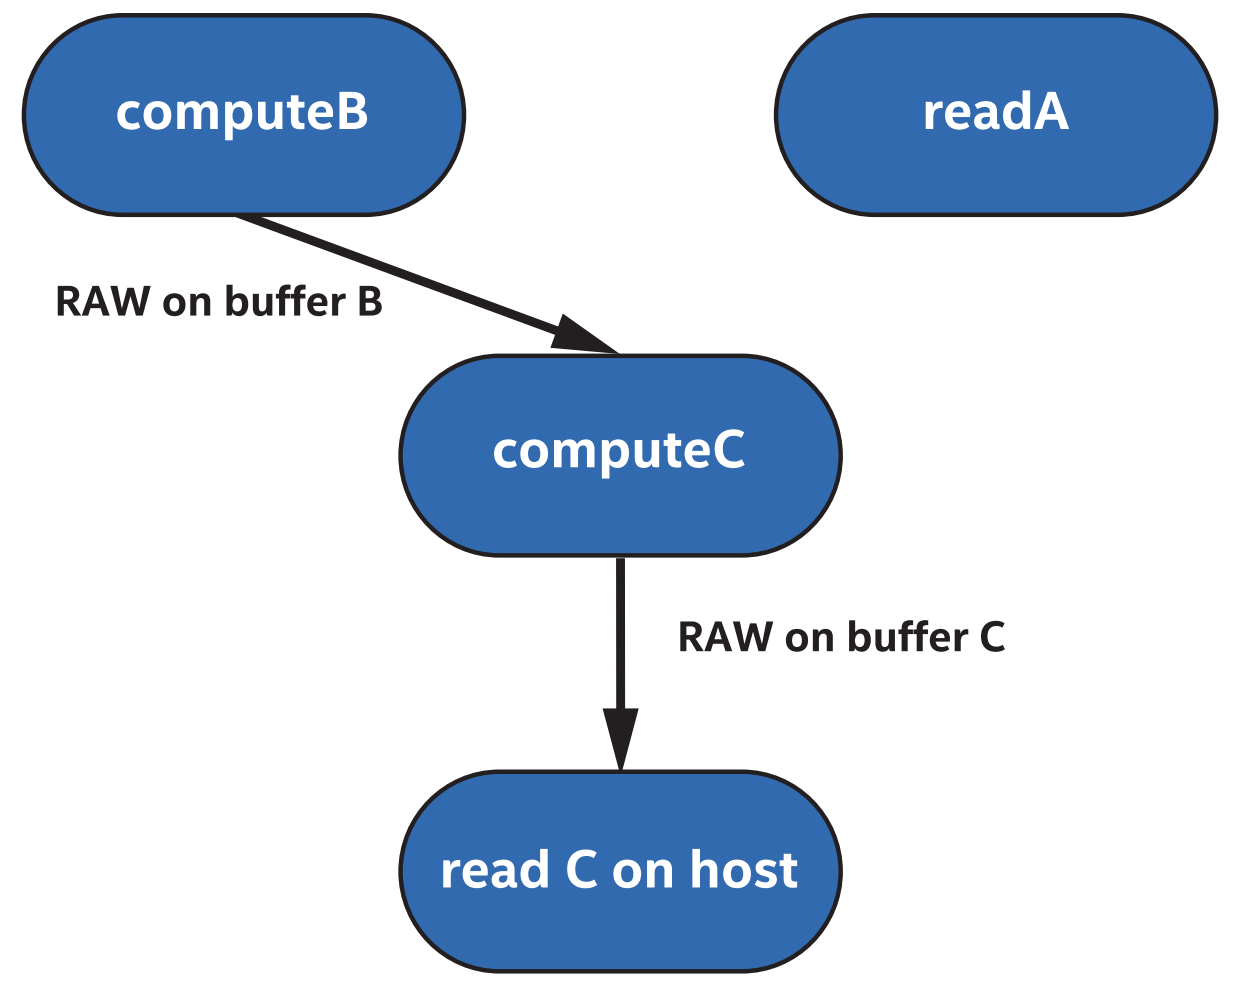
\includegraphics[width=0.6\textwidth]{content/chapter-3/images/8}
\end{center}

图3-13和图3-14中,我们执行三个内核——computeb、readA和computec——然后在主机上读取最终结果。内核computeB的命令组创建两个访问器,accA和accB。这些访问器使用访问标记read\_only和write\_only进行优化,以指定不使用默认的访问模式access::mode::read\_write。内核computeB读取缓冲区A并写入缓冲区B,缓冲区A必须在内核开始执行之前从主机复制到设备上。\par

内核readA也为缓冲区A创建一个只读访问器。因为内核readA是在内核computeB后提交的,所以这会创建一个读后读的场景。然而,读后读并没有对运行时进行限制,内核可以自由地以任何顺序执行。事实上,运行时更喜欢在内核computeB之前执行内核readA,甚至同时执行。两者都需要将缓冲区A复制到设备上,但是内核computeB也需要复制缓冲区B,以确保computeB的数据覆盖相应的缓冲区。当缓冲区B的数据传输时,运行时可以执行内核读取,即使内核只会写入缓冲区,缓冲区的原始内容仍然可移动到设备上,因为不能保证缓冲区中的所有值都由内核修改(参见第7章,关于优化标记)。\par

内核computeC读取缓冲区B,这是内核computeB计算的结果。在提交内核computeB之后,提交了内核computeC,这样内核computeC对缓冲区B有数据依赖。数据依赖也称为真依赖或流依赖,因为数据需要从计算流到另一个计算,从而计算出正确的结果。因为主机希望在内核完成后读取C,所以还在内核computeC和主机之间创建了对缓冲区C的依赖,这迫使运行时将缓冲区C复制回主机。由于设备上没有对缓冲区A的写操作,因为主机已经有了最新的数据副本,所以运行时不需要将缓冲区复制回主机。\par

\hspace*{\fill} \par %插入空行
图3-15 写后读和写后写
\begin{lstlisting}[caption={}]
#include <CL/sycl.hpp>
#include <array>
using namespace sycl;
constexpr int N = 42;

int main() {
	std::array<int,N> a, b;
	for (int i = 0; i < N; i++) {
		a[i] = b[i] = 0;
	}

	queue Q;
	buffer A{a};
	buffer B{b};
	
	Q.submit([&](handler &h) {
		accessor accA(A, h, read_only);
		accessor accB(B, h, write_only);
		h.parallel_for( // computeB
		N, [=](id<1> i) {
			accB[i] = accA[i] + 1;
		});
	});

	Q.submit([&](handler &h) {
		// WAR of buffer A
		accessor accA(A, h, write_only);
		h.parallel_for( // rewriteA
		N, [=](id<1> i) {
			accA[i] = 21 + 21;
		});
	});

	Q.submit([&](handler &h) {
		// WAW of buffer B
		accessor accB(B, h, write_only);
		h.parallel_for( // rewriteB
		N, [=](id<1> i) {
			accB[i] = 30 + 12;
		});
	});

	host_accessor host_accA(A, read_only);
	host_accessor host_accB(B, read_only);
	for (int i = 0; i < N; i++) {
		std::cout << host_accA[i] << " " << host_accB[i] << " ";
	}
	std::cout << "\n";
	return 0;
}
\end{lstlisting}

\hspace*{\fill} \par %插入空行
图3-16 写后读和写后写的任务图
\begin{center}
	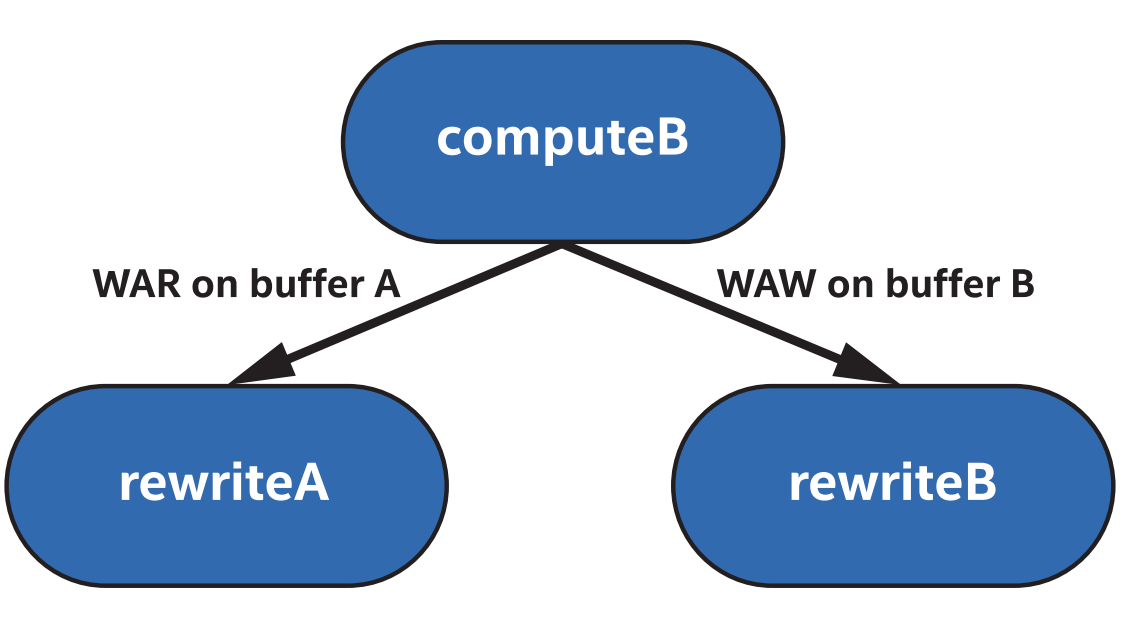
\includegraphics[width=0.6\textwidth]{content/chapter-3/images/9}
\end{center}

图3-15和3-16中,再次执行三个内核:computeB、rewriteA和rewriteB。内核rewriteA写缓冲区A,内核rewriteB写缓冲区B。内核rewriteA理论上可以比内核rewriteB更早执行,在内核准备好之前需要传输的数据更少。但必须等到内核computeB完成后,因为有一个写后读依赖于缓冲区A。\par

这个例子中,内核computeB需要从主机获取A的原始值,如果内核rewriteA在内核computeB之前执行,那将读取错误的值。写后读依赖也称为反依赖,原始依赖关系确保数据正确地流向正确的方向,而写后读依赖关系确保在读取现有值之前不会覆盖。内核重写函数中,写后写对缓冲区B的依赖与此类似。如果在内核computeB和rewriteB之间提交了任何对缓冲区B的读取,将形成读后写和写后读的依赖关系,从而正确地排序任务。然而,内核rewriteB和主机之间存在隐式的依赖关系,最终的数据必须写回主机。写后写依赖关系,也称为输出依赖关系,确保最终的输出数据在主机上的正确性。\par





















